\documentclass{article}
\usepackage[utf8]{inputenc}
\usepackage[T1]{fontenc} 
\usepackage[french]{babel}
\usepackage{graphicx}
\usepackage{subfigure}
\usepackage[table]{xcolor}
\usepackage{geometry}
\usepackage{hyperref}
\usepackage{appendix}
\usepackage{pdfpages}

\geometry{hmargin=2.5cm,vmargin=3cm}
\setlength{\parskip}{0.1cm}

\title{Rapport de Stage}
\author{Laureline MARTIN}
\date{Mercredi 7 Octobre 2020}

\begin{document}
\maketitle
\vspace*{10cm}
\begin{center}
	\textbf{Résumé :}
\end{center}
\hspace*{0.4cm}
Dans le cadre de la validation du Master 2 Data Managment in a Digital World - Datascale, proposé par l'Université de Versailles Saint-Quentin / Paris Saclay, j'ai effectué un stage de cinq mois et demi au sein du laboratoire de recherche CEDRIC du Conservatoire National des Arts et Métiers de Paris.
J'ai poursuivi ce stage en majorité en télé-travail, dû à la crise sanitaire liée à la COVID-19.
\bigskip\newline
\begin{center}
	\textbf{Abstract :}
\end{center}
\hspace*{0.4cm}
In order to validate my Master 2 Data Management in a Digital World - Datasclae by Université de Versailles Saint-Quentin / Paris Saclay, I worked for the CEDRIC research laboratory based on Conservatoire Nationnal des Arts et Métiers at Paris during five mounths and half.
Due to COVID-19 pandemic, I mostly worked at home.


\newpage
\renewcommand{\contentsname}{Table des matières}\tableofcontents

\newpage
\section{Introduction}
	Depuis quelques années, les jeux pervasifs se multiplient sur le marché, proposant aux joueurs des conetnus très immersifs.
	Le jeu pervasif (aussi appelé jeu omniprésent) est un genre de jeu qui mêle le monde physique et le monde numérique et rend floue cette frontière.
	Comme le décrit Astic dans \cite{astic_2013}, le contexte dans le jeu pervasif est essentiel. 
	Quatre facteurs sont mis en jeu : l'espace, le temps, la technologie et les rapports sociaux. 
	L'espace du jeu pervasif est à la fois ancré dans le réel et à la fois virtuel.
	Il convient alors que des ponts existent entre ces deux espaces. 
	Ces ponts peuvnet se faire via des objets, des points géographiques, des personnes, etc. 
	Le temps dans le jeu pervasif est calqué sur le temps réel mais il peut être utilisé de différentes manières. 
	L'heure et/ou le jour peuvent influencer le comportement que doit adopter le joueur.
	La technologie est également importante. Elle doit rester accessible au joueur, tant sur le plan pratique que sur le plan financier. La géolocalisation, les réseaux sans fil, etc. sont des technologies utilisées pour ce type de jeu.
	Dans les jeux pervasifs, les joueurs, les spectateurs et les non-joueurs sont mélangé sur le même espace. Les joueurs n'ont pas de caractéristiques particulières pour se reconnaître.\par
	Le projet exploratoire initié par trois enseignants-chercheurs du laboratoire CEDRIC du CNAM intitulé "Conception et développement des jeux pervasifs adaptables avec la prise en compte des états émotionnels des joueurs" vise à élaborer un jeu pervasif capable de s'adapter dynamiquement selon le contexte du joueur et son environnement. Le but est de concevoir un jeu capable de détecter et de reconnaître l'état émotionnel courant de joueur. Il faut aussi que le jeu puisse s'adapter à cet état en temps réel en proposant un événement spécifique. Cet événement devra soit maintenir le joueur dans l'état émotionnel courant, soit changer l'état émotionnel du joueur. Le choix de maintenir ou de changer l'état émotionnel du joueur devra se faire par rapport au context environnemental.
	Cependant, la conception d'un tel jeu doit rester assez générique pour pouvoir l'appliquer à d'autres domaines dans de prochains projets.\par
	J'ai rejoins ce projet à son commencement. 
	Le but de mon stage est double : 
	d'une part, je dois recueillir et synthétiser les éléments déjà existants dans la littérature scientifique et industrielle pour l'élaboration d'un tel jeu pervasif. 
	Et d'autre part, je dois élaborer un modèle conceptuel afin de représenter les éléments qui permettront par la suite d'implémenter ce jeu particularisé.\par
	Dans ce rapport, je vais tout d'abord présenter le laboratoire ainsi que l'équipe avec laquelle j'ai travaillé et son projet. Puis, je présenterai ...

\section{Cadre du stage}
	\subsection{Le laboratoire CEDRIC}
		\begin{center}
			
\includegraphics[scale=0.45]{../include/logo-cedric.PNG}\\
		\end{center}
		\hspace*{0.4cm}
		Pour ce stage, j'ai été accueillie par le laboratoire de Centre d'Etudes et De Recherche en Informatique et Communication (CEDRIC)\footnote{\href{http://cedric.cnam.fr/lab/accueil/labo/}{http://cedric.cnam.fr/lab/accueil/labo/}} au sein du Conservatoire National des Arts et Métiers (CNAM) de Paris\footnote{\href{http://www.cnam.fr/portail/accueil-conservatoire-national-des-arts-et-metiers-821166.kjsp}{http://www.cnam.fr/portail/accueil-conservatoire-national-des-arts-et-metiers-821166.kjsp}}. 
		Le laboratoire se situe au 2 rue Conte 75003 PARIS.\par
		Le laboratoire CEDRIC est composé de huit équipes ayant des actions dans le domaine de l'informatique fondamentale et appliquée, ainsi que dans d'autres disciplines proches (statistiques, électronique,...).
		\begin{itemize}
			\item L'équipe Données complexes, apprentissage et représentations (Vertigo) : Extraire de l'information et construire des méthodes de gestion de données basées sur le contenu pour des données massives audios, images et vidéos;
			\item L'équipe Interactivité pour Lire et Jouer (ILJ) : Questions autour de l'interaction homme-machine concernant des activités telles que le jeu et la lecteure. Cette équipe mèle plusieurs disciplines (informatiques, psychologie, design, arts,...) afin de répondre aux études en cours qui concernent la modélisation de la difficulté dans les jeux, les méthodologies de game design inclusif,...;
			\item L'équipe Ingénieries des Systèmes d'Information et de Décision (ISID) : Réunie autour de trois axes de recherche (les systèmes décisionnels, le web sémantique et la qualité des systèmes d'information) dans le but de concevoir des méthodes, des outils et des techniques	pour la conception et l'analyse de systèmes d'information et de décision dans tous les domaines;
			\item L'équipe Traitement du signal et architectures électroniques (LAETITIA) : Concentrée sur trois axes de recherhe : traitement du signal pour les télécommunications (recherches en lien avec les réseaux cellulaires (5G/6G) et en lien avec les problématiques de couches physique pour les réseaux faible puissance longue portée pour l'IoT), sûreté de fonctionnement des sytèmes dynémiques (recherche en automatique) et implémentation temps-réel (mise en oeuvre des algorithmes proposés par l'équipe);
			\item L'équipe Méthode Statistique de Data-Mining et Apprentissage (MSDMA) : Traitement de données et développement de modèles d'apprentissage statistiques dans le but d'extraire des information pour prise de décision;
			\item L'équipe Optimisation Combinatoire (OC) : Rassemblée autour de deux axes : la programmation mathématique et applications ainsi que les graphes et optimisation;
			\item L'équipe Réseaux et Objets Connectés (ROC) : Porte sur l'analyse et l'exploitation des nouvelles architectures réseaux et des systèmes liés à la virtualisation, à la mobilité et au développemnt des objets connectés;
			\item L'équipe Systèmes Sûrs (SYS) : Spécialisation, conception, vérification et évaluation des systèmes. Pour cela, Les recherches se font autour de trois axes : l'axe typage, sémantique et preuve, l'axe architecture logiciel, architecture systèmes et ligne de produit et l'axe vérification  et évaluation de systèmes parallèles et asynchrones.
		\end{itemize}
	\subsection{L'équipe}
		L'équipe de recherche est constituée de trois enseignants-chercheurs du CNAM travaillant dans trois équipes différentes :
		\begin{itemize}
			\item Mme Elena KORNYSHOVA, Maître de conférences travaillant au sein de l'équipe \textit{Igénieurie des systèmes d'information et de décision - ISID}, 
			\item Mme Viviane GAL, ingénieure travaillant au sein de l'équipe \textit{Interactivité pour lire et jouer - ILJ},
			\item M Eric GRESSIER-SOUDAN, professeur des universités travaillant au sein de l'équipe \textit{Réseaux et Objets Connectés - ROC}
		\end{itemize}
		Tous m'ont encadré tout au long de mon stage.

\section{Cadre du projet}
	Le projet "Conception et développement des jeux pervasifs adaptables avec la prise en compte des états émotionnels des joueurs" est un projet exploratoire du laboratoire CEDRIC.
	\subsection{Motivation et objectif}
		L'objectif gloabl de ce projet est de proposer une expérience de jeu pervasif unique où le joueur et ses émotions seraient au coeur du jeu. 
		Pour cela, le jeu doit pouvoir s'adapter au joueur en fonction du contexte global. 
		C'est-à-dire que le jeu doit pouvoir détecter et reconnaître l'état émotionnel courant du joueur,
		Il doit également pouvoir proposer l'événement le plus adapter en réponse à cet état émotionnel.\par
		Dans un premier temps, le but de ce projet est de formuler un modèle conceptuel du jeu pervasif adaptatif et dynamique basé sur les états émotionnels et sur le contexte environnent. 
		Et dans un second temps, de développer une approche d'ingénerie situationnelle du système d'information pour ce type de jeu tout en restant générique pour des applications à de multiples domaines.\newline
	\subsection{Problématique}
		L'adaptation aux émotions est un problème complexe à différents niveaux.
		Il faut tout d'abord pouvoir détecter la présence d'un état émotionnel.
		Déjà plusieurs questions ce poses comme par exemble quel outil utilisé pour la détection ?\par
		Une fois détecter, il faut pouvoir reconnaître l'état émotionnel. Quelle approche utilisée ? Quel algorithme ? Pour quel(s) état(s) ?\par
		Une fois que nous connaissons l'état émotionnel du joueur, il faut pouvoir lui proposer un événement adapté à cet état. Plusieurs problèmes se posent, faut-il proposer un événement allant dans le sens de l'état émotionnel actuel du joueur ? Ou au contraire, lui proposer un événement susptible de changer son étaté émotionnel ? Quels événements sont attachés à quels états émotionnels ?\par
		De plus, tout cela doit pouvoir se faire en temps réel pour éviter un effet de décalage entre le joueur et le jeu qui pourrait distraire le joueur et le désintéressé du jeu.\par

\section{Etat de l'art}
	\textit{Voir Annexe \ref{ann:eda}.}

\section{Utilisation des données physiologiques}
	\subsection{Capteurs}
	\subsection{Middleware Oriented Messages (MOM)}
		\subsection{Comparaison entre Apache Kafka et RabbitMQ}
		\subsection{Choix de Apache Kafka}
	\subsection{Prototype : utilisation de Kafka pour des données physiologiques}

\section{Conclusion}




\newpage
\appendix
\section{Annexe 1 : Offre de stage}\label{app:annexe1}
	\textbf{Elaboration du modèle conceptuel des jeux pervasifs adaptables avec la prise en compte des états émotionnels des joueurs}\par
	\medskip
	\textbf{Contexte :}\newline
	Le champ des jeux affectifs est nouveau. Il s’appuie sur l’intégration de nouveaux moyens à développer dans les jeux afin d’adaptabilité. [1] et [2] présentent une méthodologie unifiée pour la conception des jeux affectifs utilisant le plus tôt possible le mécanisme de boucle émotionnelle. Ils repèrent des variations à l’aide de mesures physiologiques et appliquent un modèle issu d’un ensemble construit considéré comme en relation avec les émotions. Leur étude montre combien la dimension émotionnelle de l’utilisateur est importante mais difficile à gérer.\newline
	Le profil du joueur, y compris ses émotions, impacte la conception des jeux. Afin de proposer une meilleure expérience aux joueurs et de proposer un jeu particularisé, le jeu doit être adaptable en fonction du contexte global du joueur. Nous sommes dans une approche holistique qui combine à la fois l’individu et ses émotions, et, les influences de l’entourage qui va du bâtiment lui-même à l’atmosphère que dégage le lieu. Très peu de travaux ont été faits pour la conception et le développement des jeux adaptables dynamiquement. [3] formalise le concept des jeux appliqués aux visites de musées. Ce travail modélise le jeu de visite et propose un processus d’équilibrage entre la dimension ludique et la dimension non ludique (la visite) de ce type de jeux. [3] propose des patrons de mission qui servent d’éléments réutilisables lors de la conception des jeux, mais qui ne couvrent qu’une partie du processus de conception.\par
	\textbf{Sujet :}\newline
	Il s’agit dans ce stage d’élaborer un modèle conceptuel du jeu pervasif adaptable basé sur les émotions. Ce modèle, éventuellement réalisé sous forme d’une ontologie, doit couvrir toute la variété des facteurs qui impactent le jeu tels que le profil de l’utilisateur et ses données physiologiques exprimant son état émotionnel. Cette ontologie doit être construite de façon à ce qu’elle soit adaptée à la démarche situationnelle nécessaire pour la composition dynamique du jeu.

\section{Annexe 2 - Adaptation d’un jeu pervasif particularisé basée sur l'état émotionnel et sur les caractéristiques du joueur – État de l’art}\label{ann:eda}
	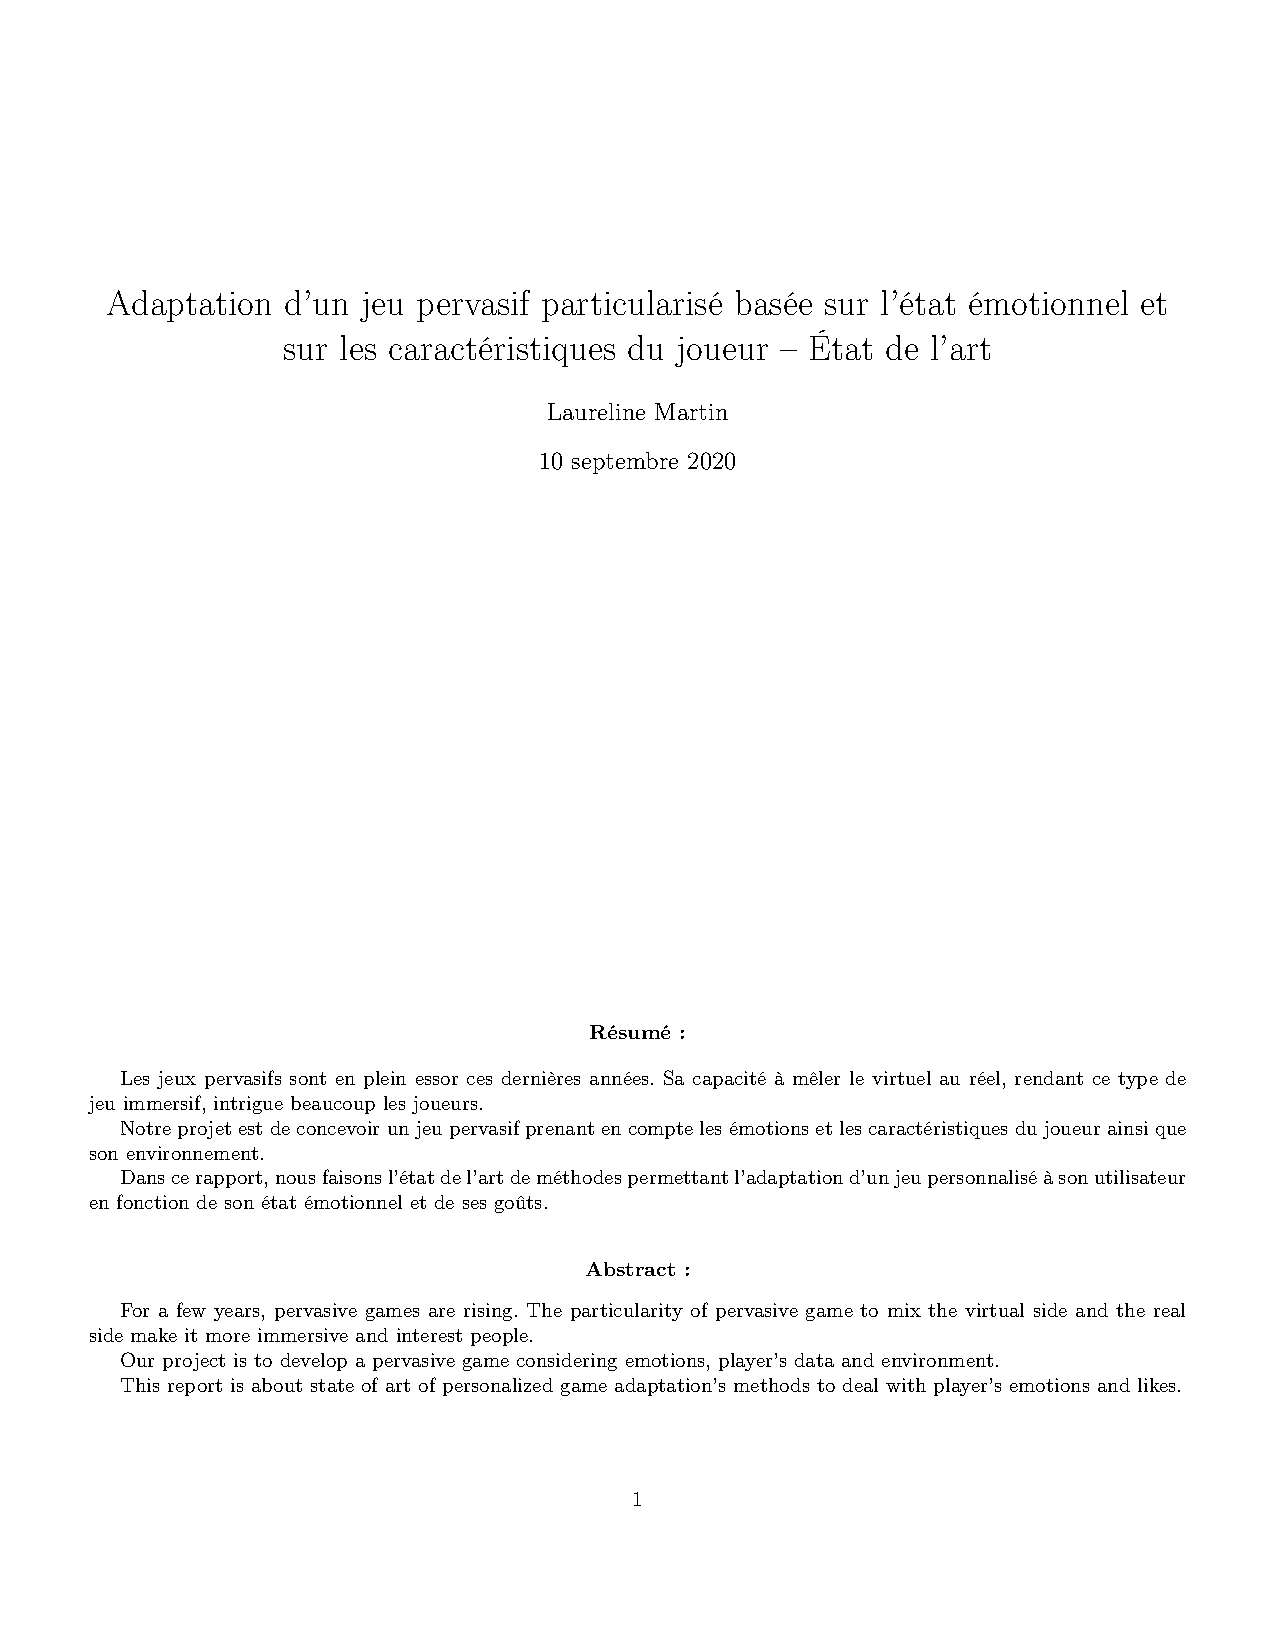
\includepdf[pages=-]{../include/eda.pdf}

%\section{Annexe 3 - Les classes en détail}\label{ann:detailclasse}
%	\includepdf[pages=-]{../include/classes.pdf}

%\section{Annexe 4 - Synthèse comparative entre Kafka et RabbitMQ}%\label{ann:kafkarabbitmq}
%	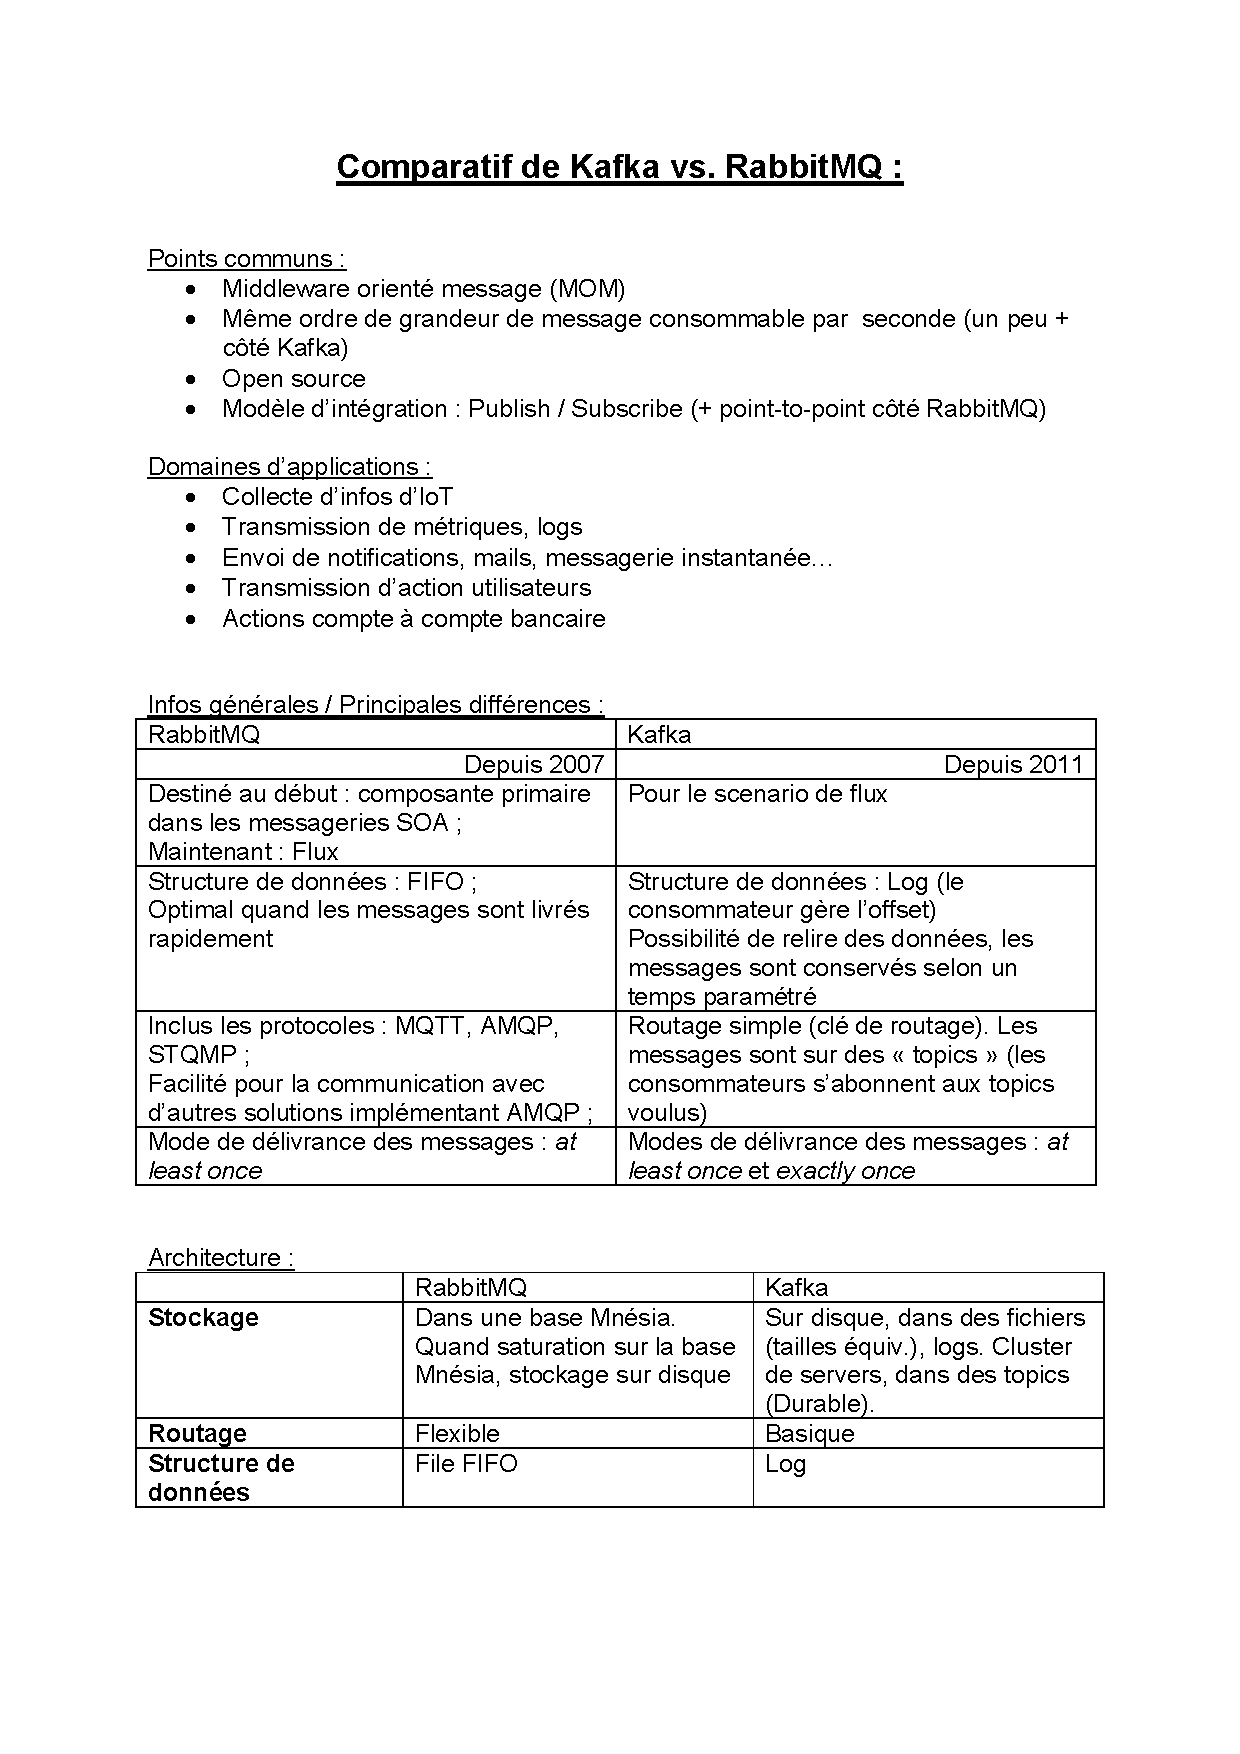
\includepdf[pages=-]{../include/comparatifKafkaVSRabbitMQ.pdf}	

\bibliographystyle{abbrv}
\bibliography{../include/biblio}
\end{document}